%!TEX root =  main.tex

\lectureheader{162}{Calculus II}{Numerical integration}{\textit{Thomas' Calculus} \textsection 8.7}

\begin{remark}\,
\begin{itemize}
\item 
%Despite all of our fancy new techniques of integration, 
Most functions do not have elementary antiderivatives, and so the fundamental theorem of calculus (part II) is practically useless for evaluating such integrals.
\item In fact, it is quite often the case that the only antiderivative that we know is the one that we ``invent" using the fundamental theorem of calculus (part I).
\item For example, our favorite antiderivative for $f(x)=1/x$ is 
\begin{equation*}
\ln x = \int_1^x\frac{\dee t}{t} \quad (x>0).
\end{equation*}
\item When asked to evaluate $\int_1^2\frac{\dee t}{t}$, we usually say that
\begin{equation*}
\int_1^2\frac{\dee t}{t} = \ln t\Big|_1^2 = \ln 2,
\end{equation*}
but that is really just a cop-out. 
\item After all what is $\ln 2$?  That answer is merely the name that we have given to $\int_1^2\frac{\dee t}{t}$.
\item A lot of functions are ``invented" using the fundamental theorem of calculus (part I).
\begin{enumerate}
\item The \textbf{error function} is defined to be a certain antiderivative of $f(x) = \frac{2}{\sqrt\pi}\E^{-x^2}$, namely
\begin{equation*}
\erf (x) = \frac{2}{\sqrt\pi}\int_0^x\E^{-t^2}\dee t.
\end{equation*}
\item The \textbf{sine integral} is defined to be a certain antiderivative of $\sinc(x) = \frac{\sin x}{x}$, namely
\begin{equation*}
\Si(x) = \int_0^x\frac{\sin t}{t}\dee t.
\end{equation*}
This one is an improper integral even!
\item The \textbf{logarithmic integral} is defined to be a certain antiderivative of $f(x) = 1/\ln (x)$, namely
\begin{equation*}
\Li(x) = \int_0^x\frac{\dee t}{\ln t}.
\end{equation*}
This one is doubly improper!
%\item The \textbf{gamma function} is a-whole-nother story
%\begin{equation*}
%\Gamma(x) = \int_0^\infty t^{x-1}\E^{-t}\dee t.
%\end{equation*}
\end{enumerate}
\end{itemize}
\end{remark}


\begin{remark}\,
\begin{itemize}
\item Another problem with integration (as we have learned it so far) is that not all functions that we meet in ``real life" have neat formulas.
\item Sometimes we just have laboratory data $(x_0, y_0), \dots, (x_n,y_n)$, and we don't know the value of $f(x)$ at points between $x_{i-1}$ and $x_i$ without running more experiments or building another prototype.
\item No matter how many experiments we do, we only get to know the value of $f(x)$ at \textit{finitely many} points.
\end{itemize}
\end{remark}

\begin{definition}[Trapezoidal rule]
Let $[a,b]$ be a finite length interval, and let $f$ be continuous on $[a,b]$.
\begin{itemize}
\item Partition the interval $[a,b]$ into $n$ equal length pieces
\begin{equation*}
a=x_0 < x_1 <\dots < x_{n-1} < x_n = b,
\end{equation*}
where $\Delta x = x_i - x_{i-1} = \frac{b-a}{n}$ for $i=1,\dots, n$.
\item For $i=0,1,\dots, n$, evaluate $y_i = f(x_i)$.
\end{itemize}
The \textbf{trapezoidal approximation} is
\begin{equation*}
\begin{split}
\int_a^bf(x)\dee x &\approx \frac{\Delta x}{2}\left[y_0 + 2\sum_{i=1}^{n-1} y_i + y_n\right]\\
&= \frac{\Delta x}{2}\Big(y_0 + 2y_1 + \dots + 2y_{n-1} + y_n\Big).
\end{split}
\end{equation*}
\end{definition}

\begin{remark}\,
\begin{itemize}
\item The idea idea behind the trapezoidal rule is to approximate $f(x)$ (or the discrete data) on the subinterval $[x_{i-1}, x_i]$ by linear interpolation.
\item In particular, the unique linear polynomial $p_i(x)$ passing through the data $(x_{i-1}, y_{i-1})$ and $(x_i, y_i)$ is
\begin{equation*}
p_i(x) = y_{i-1} + m_i(x-x_{i-1}),
\end{equation*}
where $m_i = \frac{y_i - y_{i-1}}{x_i-x_{i-1}} = \frac{\Delta y_i}{\Delta x}$.
\item Note then that
\begin{equation*}
\int_{x_{i-1}}^{x_i} p_i(x)\dee x
%= y_{i-1}x + \frac{m_i}{2}(x-x_{i-1})^2\Big|_{x_{i-1}}^{x_i}
%&= y_{i-1}(x_i - x_{i-1}) + \frac{m_i}{2}(x_i-x_{i-1})^2\\
%&= y_{i-1}\Delta x +\frac{m_i}{2}\Delta x^2\\
%&= \frac{\Delta x}{2}\left(2y_{i-1} +m_i\Delta x\right)\\
 = \frac{\Delta x}{2}\left( y_i + y_{i-1}\right),
\end{equation*}
the area of the trapezoid under the line $y=p_i(x)$.
\begin{figure}[H]
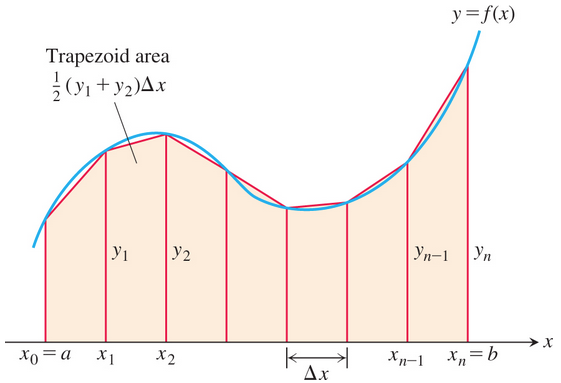
\includegraphics[height=2.5in]{img/trapezoidal_rule}
\end{figure}
\item  Therefore,
\begin{equation*}
\int_a^bf(x)\dee x 
= \sum_{i=1}^n\int_{x_{i-1}}^{x_i} f(x)\dee x
\approx \sum_{i=1}^n\int_{x_{i-1}}^{x_i} p_i(x)\dee x
= \frac{\Delta x}{2}\sum_{i=1}^n\left(y_i+y_{i-1}\right).
\end{equation*}
\end{itemize}
\end{remark}


\newpage

\begin{example}
Use the trapezoidal rule with $n=6$ to estimate $\ln 2$.
\end{example}

\newpage

\begin{remark}
When the second derivative $f''$ is continuous on $[a,b]$, we can use the following theorem to bound the error in the trapezoidal approximation.
\end{remark}

\begin{theorem}
Suppose $f''$ is continuous on $[a,b]$ and that $|f''(x)|\le M$ for all $x\in [a,b]$.
If $E_T$ is the error in the $n$-step  trapezoidal approximation of $\int_a^bf(x)\dee x$, then
\begin{align*}
%|E_M| &\le \frac{M(b-a)^3}{24n^2},\\
|E_T| &\le \frac{M(b-a)^3}{12n^2}.
\end{align*}
\end{theorem}

\begin{example}
Use the above to bound the error in the trapezoidal approximation of $\ln 2$ when $n=6$.
How large must $n$ be to ensure that the error is less than $10^{-6}$?
\end{example}

\newpage

\begin{remark}\,
\begin{itemize}
\item In some situations, Simpson's approximation achieves ``faster" convergence by using a quadratic interpolation.
\item Just as we need 2 points to determine a line, we need 3 to determine a parabola.
\item As a consequence, we must partition the interval $[a,b]$ into an even number of pieces.
\end{itemize}
\end{remark}

\begin{figure}[H]
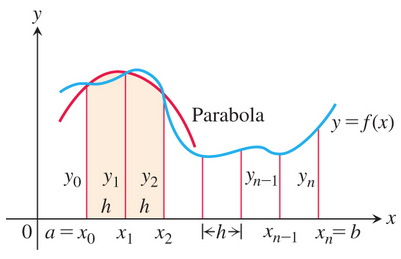
\includegraphics[height=2.5in]{img/simpson_rule}
\end{figure}

\begin{definition}[Simpson's rule]
Let $[a,b]$ be a finite length interval, and let $f$ be continuous on $[a,b]$.
\begin{itemize}
\item Partition the interval $[a,b]$ into $n=2m \ge 2$ (an even number of) equal length pieces
\begin{equation*}
a=x_0 < x_1 <\dots < x_{n-1} < x_n = b,
\end{equation*}
where $\Delta x = x_i - x_{i-1} = \frac{b-a}{n}$ for $i=1,\dots, n$.
\item For $i=0,1,\dots, n$, evaluate $y_i = f(x_i)$.
\end{itemize}
\textbf{Simpson's approximation} is
\begin{equation*}
\begin{split}
\int_a^bf(x)\dee x &\approx \frac{\Delta x}{3}\left[y_0 + 4\sum_{i=0}^{m-1} y_{2i+1} + 2\sum_{i=1}^{m-1} y_{2i} + y_n\right]\\
&= \frac{\Delta x}{3}\Big(y_0 + 4y_1 + 2y_2 + \dots + 2y_{n-2} + 4y_{n-1} + y_n\Big).
\end{split}
\end{equation*}
\end{definition}

\newpage

\begin{example}
Use Simpson's rule with $n=6$ to estimate $\ln 2$.
\end{example}

\newpage

\begin{theorem}
Suppose $f^{(4)}$ is continuous on $[a,b]$ and that $|f^{(4)}(x)|\le M$ for all $x\in [a,b]$.
If $E_S$ is the $n$-step error in Simpson's approximation of $\int_a^bf(x)\dee x$, then
\begin{equation*}
|E_S| \le \frac{M(b-a)^5}{180n^4}.
\end{equation*}
\end{theorem}



\begin{example}
Use the above to bound the error in Simpson's approximation of $\ln 2$ when $n=6$.
How large must $n$ be to ensure that the error is less than $10^{-6}$?
\end{example}
